\documentclass{beamer}

\usetheme{simple}

\usepackage{scalerel,xparse}
\usepackage{lmodern}
\usepackage[scale=2]{ccicons}
\usepackage{ulem}
\usepackage{tikz}
\usetikzlibrary{positioning,calc,automata}
\usepackage{algorithm}
\usepackage{algorithmic}
\usepackage{caption}
\usepackage{listings}

% Watermark background (simple theme)
\setlength{\parindent}{0cm}
\setwatermark{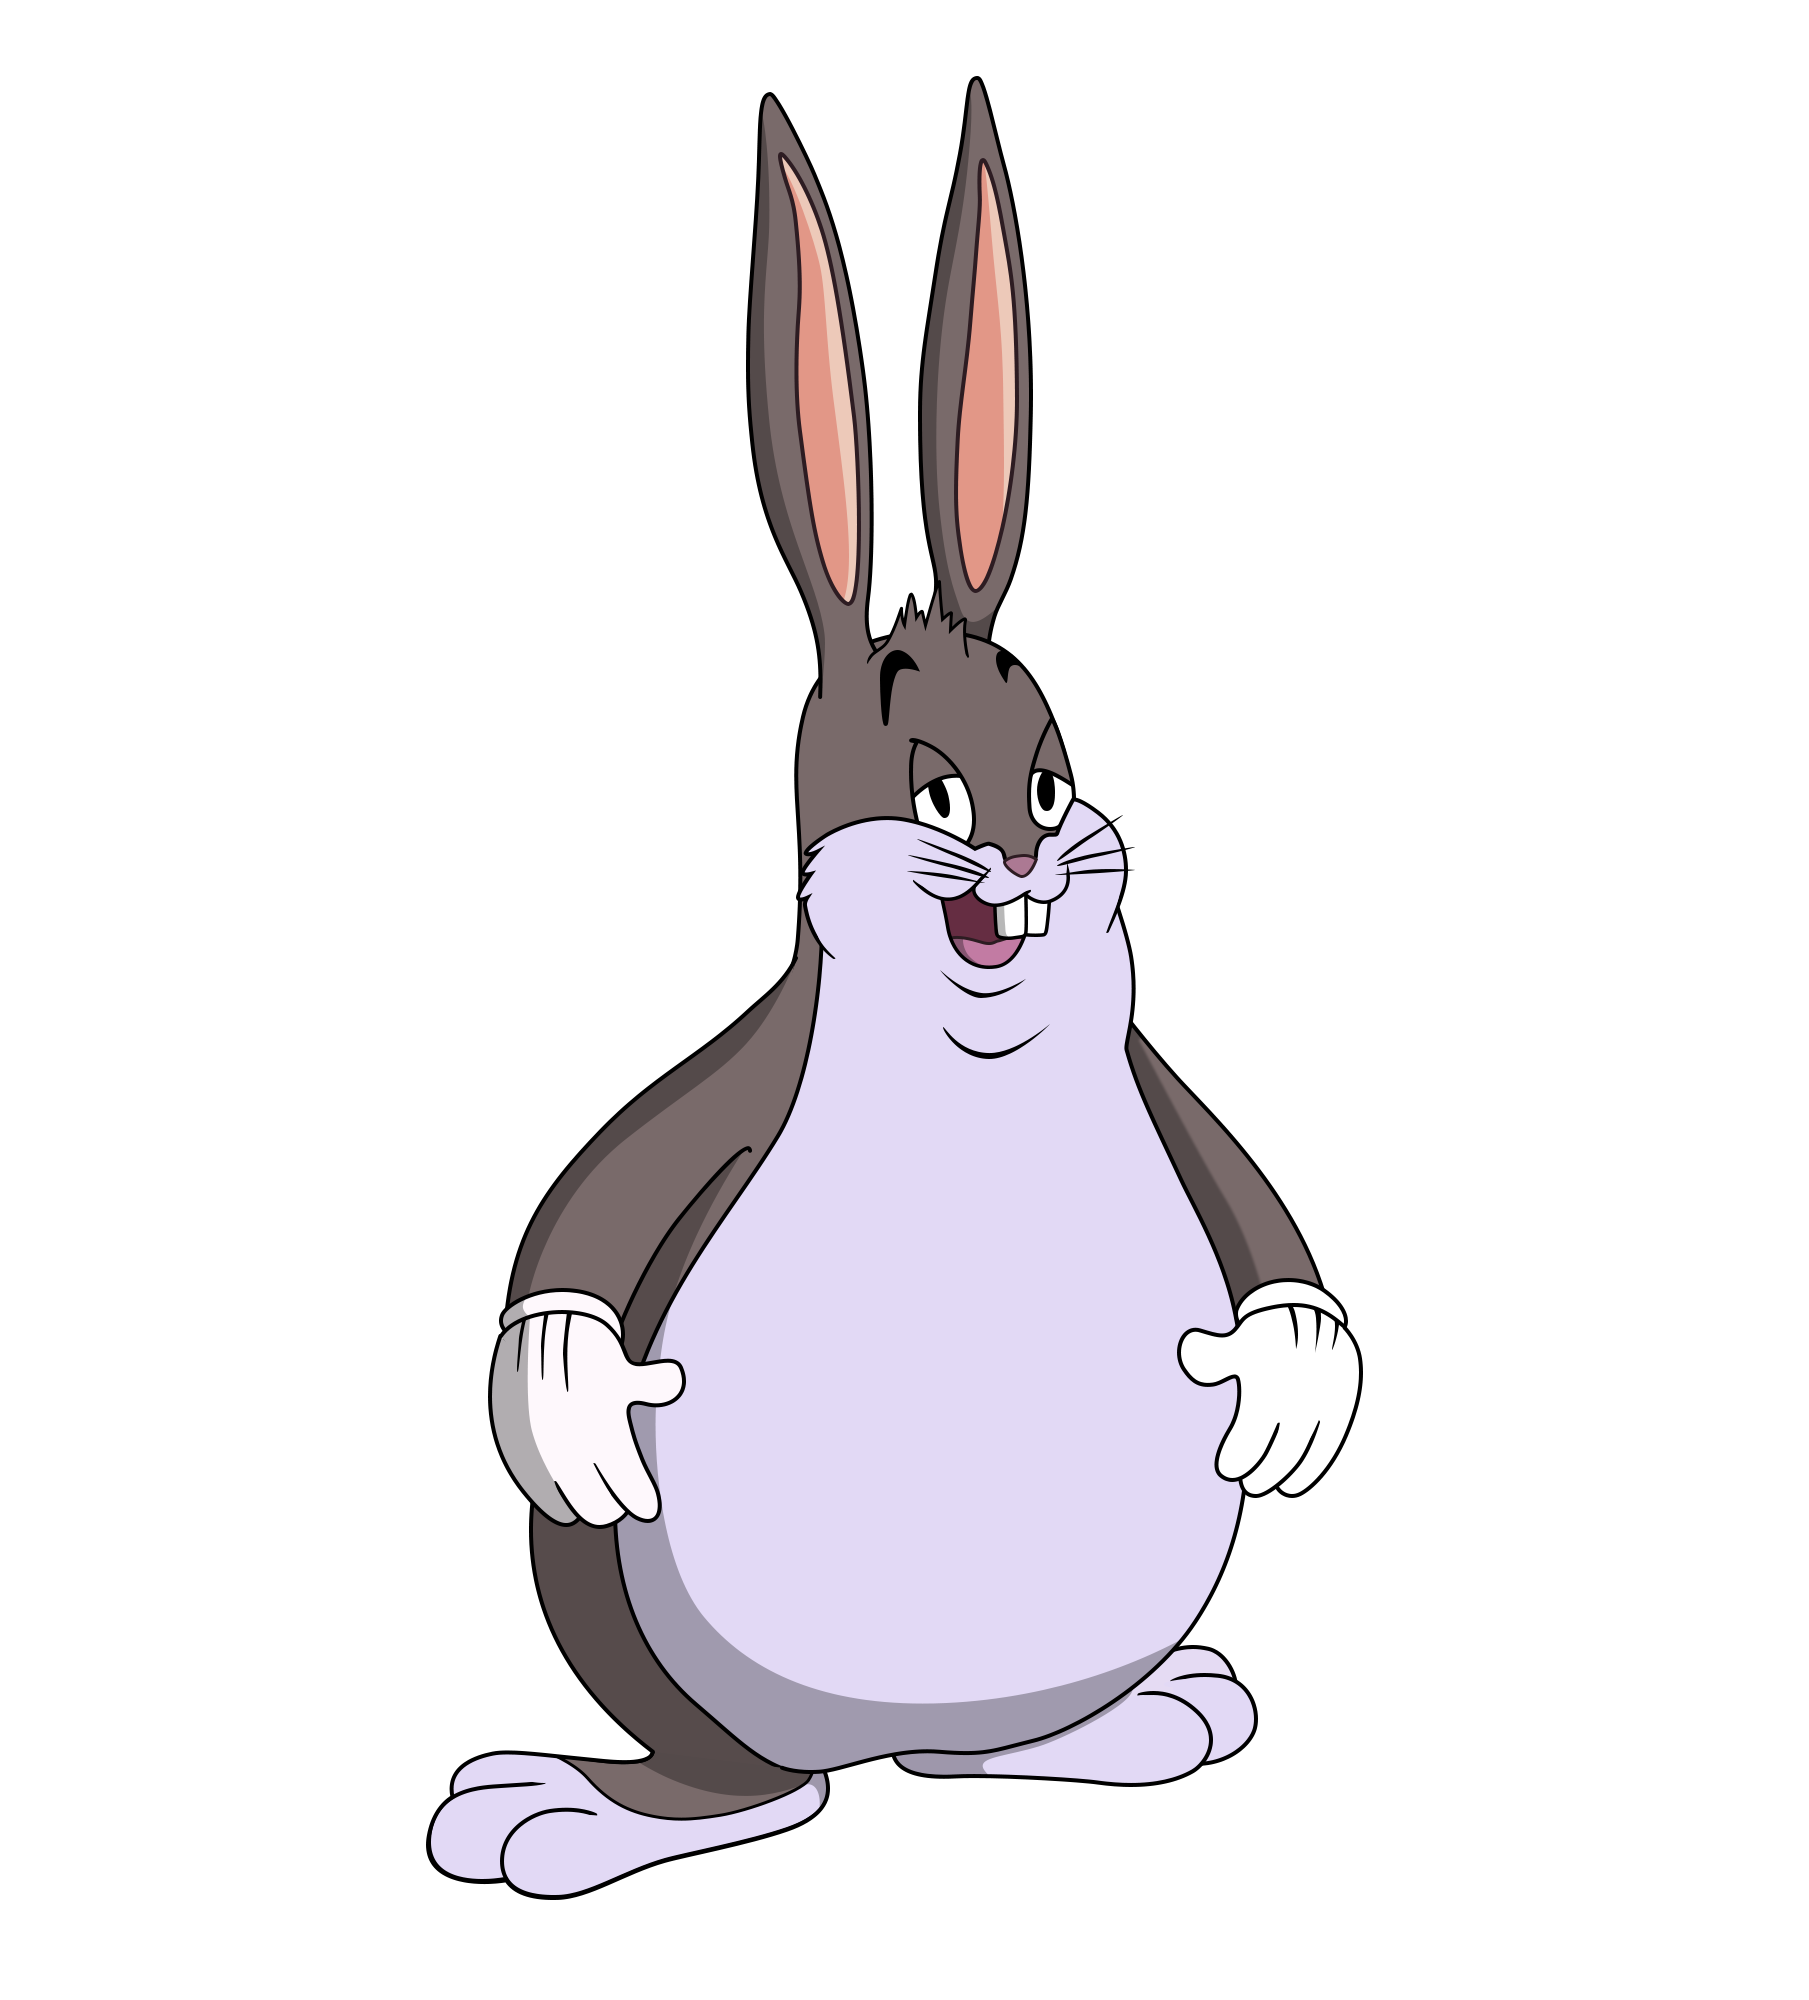
\includegraphics[height=8cm]{img/chungus.png}}


\title{CSC363H5 Tutorial 3}
\subtitle{I'm back!!! yay}
\date{\today}
\author{Paul ``sushi{\textunderscore}enjoyer'' Zhang}
\institute{University of Chungi}

\NewDocumentCommand\emojisushi{}{
    
\includegraphics{img/1f363.png}
}
\NewDocumentCommand\emojimoyai{}{
    
\includegraphics{img/1f5ff.png}
}
\NewDocumentCommand\emojicroissant{}{
    
\includegraphics[scale=0.07]{img/1f950.png}
}
\NewDocumentCommand\emojiknife{}{
    
\includegraphics[scale=0.05]{img/1f52a.png}
}
\NewDocumentCommand\emojihearteyes{}{
    
\includegraphics[scale=0.05]{img/1f60d.png}
}
\NewDocumentCommand\emojitriumph{}{
    
\includegraphics[scale=0.8]{img/1f624.png}
}

\begin{document}

\maketitle

\begin{frame}{Learning objectives this tutorial}
By the end of this tutorial, you should...
\begin{itemize}
\item Be fully convinced that Turing computability is much easier to understand than G*del computability.
\item Have a list of synonyms for ``computable'' and ``partial computable''.
\item Have a complete, mathematically-rigorous proof of the very intuitive fact that you can label things with numbers.
\item Convince yourself to never take MAT309. To scare you even more, here's a proof I wrote in that course (page 1/3):
\begin{figure}[h]
\centering
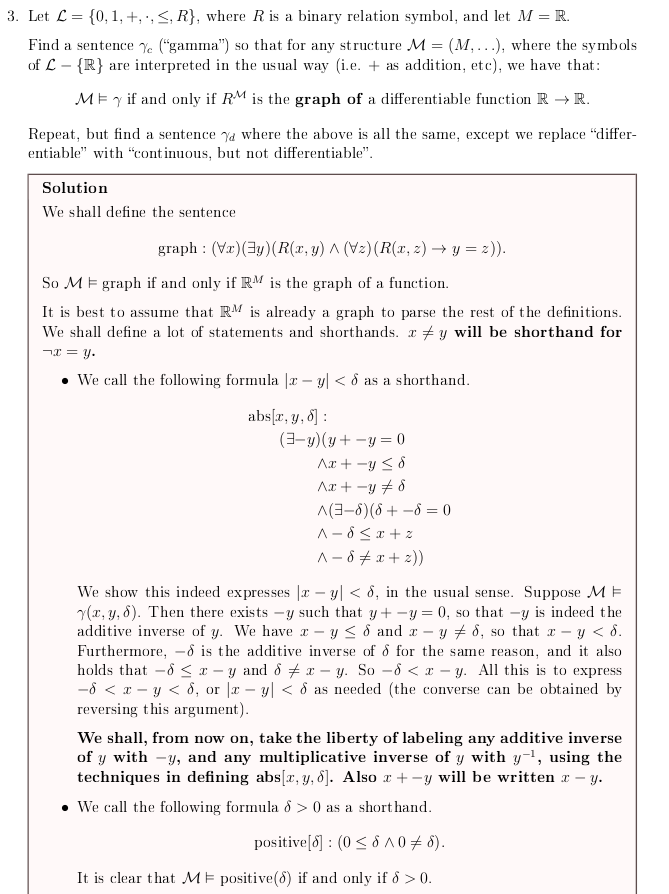
\includegraphics[scale=0.1]{img/309.png}
\end{figure}
\end{itemize}
\end{frame}

\begin{frame}{Quiz 2 is administered in this tutorial.\footnote{no it isn't, but stay tuned!}}
\textbf{Question 1 (1 point):} Do you hate Turing machines?

\vspace{20mm}

\textbf{Question 2 (1 point):} Do you like partial recursive functions?

\vspace{20mm}

\textbf{Question 3 (1 point):} Have you finished Assignment 1?
\end{frame}

\begin{frame}{Answer key}
\textbf{Question 1 (1 point):} Do you hate Turing machines?

\textbf{Answer}: yep, i hate Turing machines!\emojiknife

\vspace{15mm}

\textbf{Question 2 (1 point):} Do you like partial recursive functions?

\textbf{Answer}: yes! they are so much better than Boring machines.\emojihearteyes

\vspace{15mm}

\textbf{Question 3 (1 point):} Have you finished Assignment 1?

\textbf{Answer}: yes! i love doing csc363 homework \emojitriumph
\end{frame}

\begin{frame}{let's review some words!}
\textbf{Task:} List all synonyms of \textit{computable} you have encountered so far in this course.

\textbf{Task:} List all synonyms of \textit{partial computable} you have encountered so far in this course.

\begin{figure}[h]
\centering

\includegraphics[scale=0.3]{img/dontstop.jpg}
\end{figure}
\end{frame}

\begin{frame}{let's review some words!}
\textbf{Task:} List all synonyms of \textit{computable} you have encountered so far in this course.

\textbf{Answer:} \textit{decidable}, \textit{nice}, \textit{not weird}, \textit{won't take forever to decide whether something is in it or not}

\vspace{15mm}

\textbf{Task:} List all synonyms of \textit{partial computable} you have encountered so far in this course.

\textbf{Answer:} \textit{listable}, \textit{computably enumerable (c.e.)}, \textit{partial recursive}, \textit{Diophantine}, \textit{the reason why we are spending weeks on material you'll probably never see in a software job}


\vspace{20mm}

Note: \textit{primitive recursive} is neither of those. 
\end{frame}

\begin{frame}{the reason why you're here today...}
is to prove this one statement!

\vspace{20mm}

\begin{quotation}
If $A \subseteq \mathbb N$ is an infinite computable set, then there exists an injective computable function $f: \mathbb N \to \mathbb N$ such that $A$ is the range of $f$.
\end{quotation}
\begin{flushright}
- professor \texttt{helo\textunderscore fish.jpg}, probably, 2021\\
\end{flushright}

Oh wait, \texttt{helo\textunderscore fish.jpg} is back! she is no longer sad and feeling quite flushed right now.

\end{frame}

\begin{frame}{\texttt{helo\textunderscore fish\textunderscore flushed.jpg}}

\begin{figure}[h]
\centering

\includegraphics[scale=0.3]{img/helo_fish_flushed.jpg}

mmm... idk, happy early valentines day i guess? ;-;

(btw, sowwy i couldn't hold tutorial last week!)
\end{figure}

\texttt{helo\textunderscore fish\textunderscore flushed.jpg} wants to grant you one wish. Of course your wish is to know what an infinite computable set is! Say ``\texttt{helo\textunderscore fish\textunderscore flushed.jpg}, what is an infinite computable set?''

\end{frame}

\begin{frame}{\texttt{helo\textunderscore fish\textunderscore flushed.jpg}}

\begin{figure}[h]
\centering
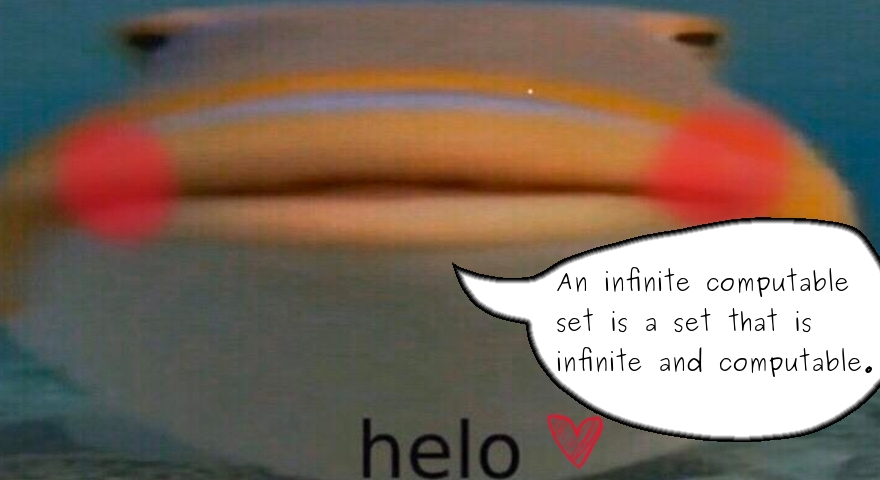
\includegraphics[scale=0.3]{img/helo_fish_ic.jpg}

bruh.
\end{figure}

Okay, now \texttt{helo\textunderscore fish\textunderscore flushed.jpg} can go since she has granted your wish. Say goodbye to \texttt{helo\textunderscore fish\textunderscore flushed.jpg}!
\end{frame}

\begin{frame}{Okay question time.}

\begin{figure}[h]
\centering
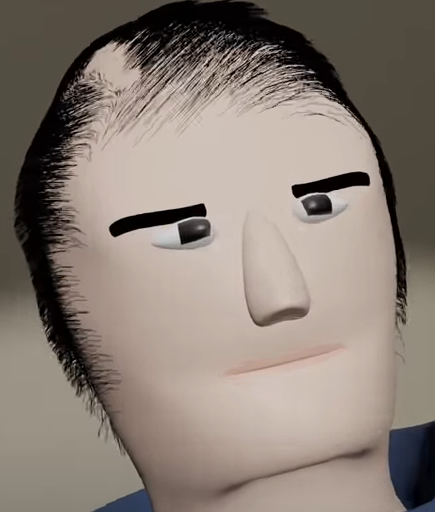
\includegraphics[scale=0.2]{img/bench_appearo.png}
\end{figure}

In fact, we only need partial computability:

\vspace{2mm}

If $A \subseteq \mathbb N$ is an infinite \sout{computable} partial computable set, then there exists an injective computable function $f: \mathbb N \to \mathbb N$ such that $A$ is the range of $f$.

\vspace{2mm}

\textbf{Task:} Prove this. (5 mins)
\end{frame}

\begin{frame}{Okay question time.}

\begin{figure}[h]
\centering
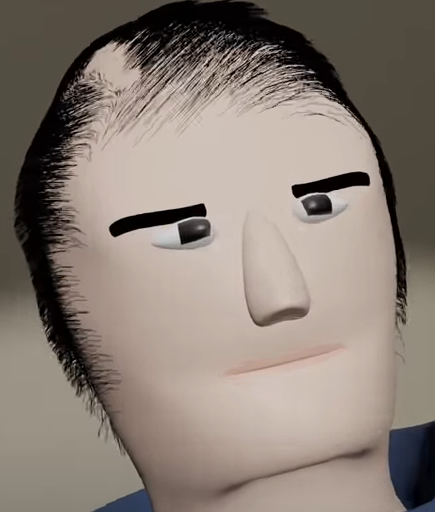
\includegraphics[scale=0.2]{img/bench_appearo.png}
\end{figure}

In fact, we only need partial computability:

\vspace{2mm}

If $A \subseteq \mathbb N$ is an infinite \sout{computable} partial computable set, then there exists an injective computable function $f: \mathbb N \to \mathbb N$ such that $A$ is the range of $f$.

\vspace{2mm}

\sout{\textbf{Task:} Prove this. (5 mins)}

I'll lead you through the proof instead, because again, Greek letters spook people.

\textbf{Task:} Read and understand the statement to keep in your head (1-2 min).
\end{frame}

\begin{frame}{Okay question time.}

Recall: if $A \subseteq \mathbb N$ is partial computable, then there exists a \textbf{computable} function $f: \mathbb N \to \mathbb N$ such that $A$ is the range of $f$. (but $f$ might not be injective!)

\vspace{2mm}

In other words,
$$A = \{f(0), f(1), f(2), \ldots\}$$
(but there may be repeats in the above list, as $f$ might not be injective!)

\vspace{2mm}

Our task is to find an \textit{injective} function $h: \mathbb N \to \mathbb N$ such that
$$A = \{h(0), h(1), h(2), \ldots\}$$
(the above list can't have repeats!)
\end{frame}

\begin{frame}{How do we remove repeats intuitively?}
Say $A$ is the set of odd numbers, and $f$ was some weird function that wanted to enumerate all the odd numbers, but really likes the number $69$.
$$A = \{69, 1, 69, 3, 69, 5, 69, 7, \ldots\} = \{f(0), f(1), f(2), f(3), \ldots\}$$

\textbf{Task:} How would you make an injective function $h$ that generates the same set, but without repeats? (Don't need you to be formal here, just describe what to do)
\end{frame}

\begin{frame}{How do we remove repeats intuitively?}
\textbf{Task:} How would you make an injective function $h$ that generates the same set, but without repeats? (Don't need you to be formal here, just describe what to do)

\vspace{2mm}

\textbf{Answer:} Choose $h(n)$ to be the $n$th\footnote{Technically $A$ is a \textit{set} and doesn't have an ``$n$th element'' since sets don't have an order. But we can order $A$ like $f(0), f(1), \ldots$} element that hasn't been listed yet.
$$A = \{69, 1, 69, 3, 69, 5, 69, 7, \ldots\} = \{f(0), f(1), f(2), f(3), \ldots\}$$
In this case, $h(0) = 69$, $h(1) = 1$, $h(2) = 3$, $h(3) = 5$, and so on. 

\vspace{2mm}

Now we just have to formalize the definition of $h$.
\end{frame}

\begin{frame}{How do we remove repeats intuitively?}
$$A = \{69, 1, 69, 3, 69, 5, 69, 7, \ldots\} = \{f(0), f(1), f(2), f(3), \ldots\}$$
In this case, $h(0) = 69$, $h(1) = 1$, $h(2) = 3$, $h(3) = 5$, and so on. 

\vspace{2mm}

So to construct such an $h$, we have
$$h(0) = f(0)$$
$$h(n + 1) = f(k),$$ where $k$ is the minimal integer such that $f(k) \notin \{h(0), h(1), \ldots, h(n)\}$.

\textbf{Task:} Make sense of why the above works by trying to apply it on the example I gave.
\end{frame}

\begin{frame}{Some building blocks first!}

Suppose we have defined $h(0), h(1), \ldots, h(n)$ already, and we want to define $h(n + 1)$. For $n \in \mathbb N$, Let $$S_n = \{h(m): m \leq n\} = \{h(0), h(1), \ldots, h(n)\}.$$

\vspace{2mm}

\textbf{Task:} Why is $S_n$ a computable set for any $n \in \mathbb N$?


\end{frame}

\begin{frame}{Some building blocks first!}

Suppose we have defined $h(0), h(1), \ldots, h(n)$ already, and we want to define $h(n + 1)$. For $n \in \mathbb N$, Let $$S_n = \{h(m): m \leq n\} = \{h(0), h(1), \ldots, h(n)\}.$$

\vspace{2mm}

\textbf{Task:} Why is $S_n$ a computable set for any $n \in \mathbb N$?

\textbf{Answer:} $S_n$ is finite for any $n$, and finite sets are always computable (according to professor Chungus).

\end{frame}

\begin{frame}{Some building blocks first!}

Suppose we have defined $h(0), h(1), \ldots, h(n)$ already, and we want to define $h(n + 1)$. For $n \in \mathbb N$, Let $$S_n = \{h(m): m \leq n\} = \{h(0), h(1), \ldots, h(n)\}.$$

\vspace{2mm}

\textbf{Task:} Why is the following function $g: \mathbb N \times \mathbb N \to \mathbb N$ computable? (Give a Turing machine argument)
$$g(n, k) = \begin{cases}
0 & f(k) \notin S_n\\
1 & f(k) \in S_n
\end{cases}$$

\end{frame}

\begin{frame}{Some building blocks first!}

Suppose we have defined $h(0), h(1), \ldots, h(n)$ already, and we want to define $h(n + 1)$. For $n \in \mathbb N$, Let $$S_n = \{h(m): m \leq n\} = \{h(0), h(1), \ldots, h(n)\}.$$

\vspace{2mm}

\textbf{Task:} Why is the following function $g: \mathbb N \times \mathbb N \to \mathbb N$ computable? (Give a Turing machine argument)
$$g(n, k) = \begin{cases}
0 & f(k) \notin S_n\\
1 & f(k) \in S_n
\end{cases}$$

\textbf{Answer:} Just check if $f(k) = f(0)$ or $f(k) = f(1)$ or $f(k) = f(2)$, until $f(k) = f(n)$.

\end{frame}

\begin{frame}{I hope you remember how to pronounce this Greek letter!}

\textbf{Task:} Pronounce the following Greek letter: $\mu$

\vspace{5mm}

\textbf{Task:} What does $\mu y[g(\overline{x}, y) = 0]$ represent? (I've forgotten too, dw)

\end{frame}

\begin{frame}{I hope you remember how to pronounce this Greek letter!}

\textbf{Task:} Pronounce the following Greek letter: $\mu$

\textbf{Answer:} $\mu$ 

\begin{figure}[h]
\centering
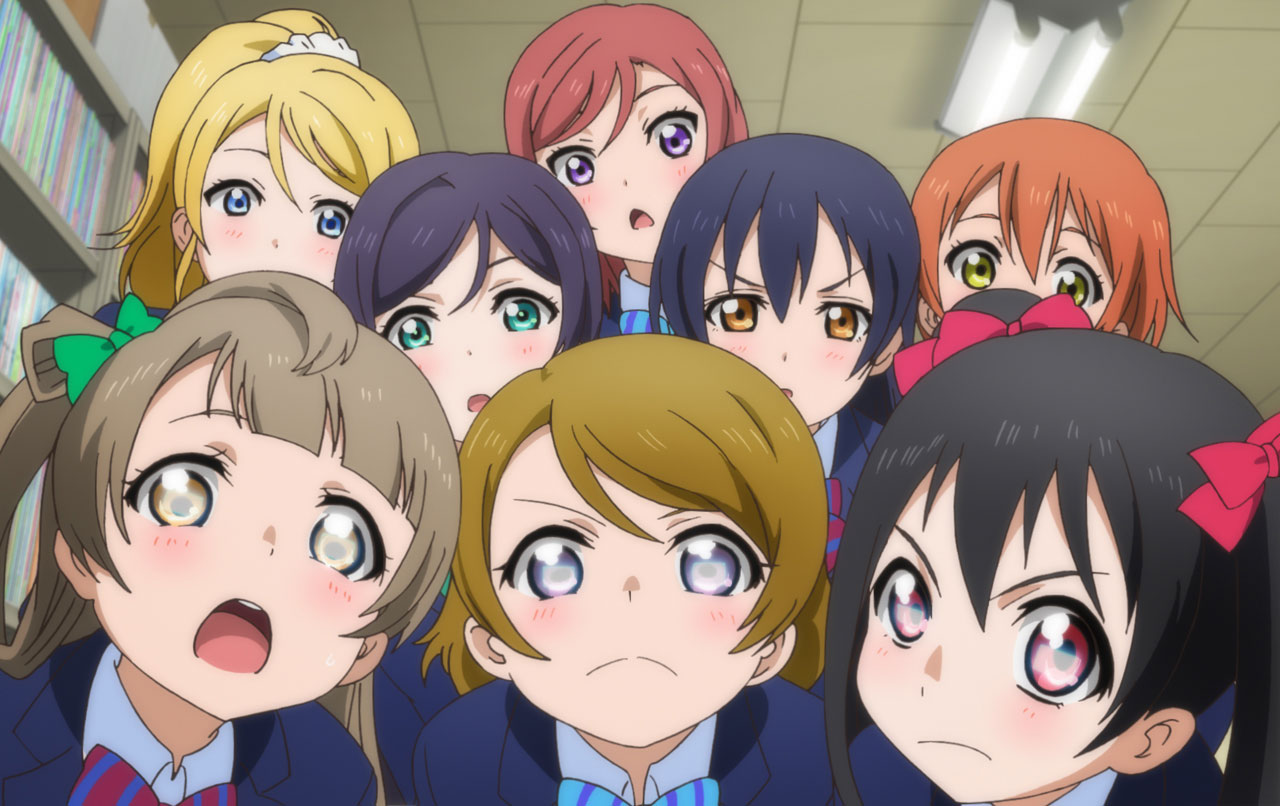
\includegraphics[scale=0.1]{img/muse.jpg}

(i only remember $\mu$'s from love live school idol project lol)

(and no, i don't really like this anime)
\end{figure}

\textbf{Task:} What does $\mu y[g(\overline{x}, y) = 0]$ represent? (I've forgotten too, dw)
\textbf{Answer:} $\mu y[g(\overline{x}, y) = 0]$ is the \textbf{minimum $y \in \mathbb N$} such that $g(\overline{x}, y) = 0$. (This minimum might not exist! in which case this is left undefined)

\end{frame}

\begin{frame}{I hope you remember how to pronounce this Greek letter!}

Recall: $$S_n = \{h(m): m \leq n\} = \{h(0), h(1), \ldots, h(n)\}$$ $$g(n, k) = \begin{cases}
0 & f(k) \notin S_n\\
1 & f(k) \in S_n.
\end{cases}$$

\textbf{Task:} (in words) What is $\mu k[g(n, k) = 0]$?

\end{frame}

\begin{frame}{I hope you remember how to pronounce this Greek letter!}

Recall: $$S_n = \{h(m): m \leq n\} = \{h(0), h(1), \ldots, h(n)\}$$ $$g(n, k) = \begin{cases}
0 & f(k) \notin S_n\\
1 & f(k) \in S_n.
\end{cases}$$

\textbf{Task:} (in words) What is $\mu k[g(n, k) = 0]$?

\textbf{Answer:} $\mu k[g(n, k) = 0]$ is the first $k \in \mathbb N$ such that $f(k) \notin S_n$. 

\vspace{4mm}

But remember, we wanted to set $h(n + 1) = f(k)$ where $k$ is the first integer with $f(k) \notin S_n$! So we can let
$$h(n + 1) = f(\mu k[g(n, k) = 0]).$$

\end{frame}

\begin{frame}{We can formalize this now.}

We have:
$$h(0) = f(0)$$
$$h(n + 1) = f(\mu k[g(n, k) = 0]).$$

Recall: if $f_1$ and $f_2$ are partial recursive, and
$$F(x, 0) = f_1(x)$$
$$F(x, s(n)) = f_2(x, n, F(x, n))$$
then $F$ is partial recursive.
\end{frame}

\begin{frame}{We can formalize this now.}

We have:
$$h(0) = f(0)$$
$$h(n + 1) = f(\mu k[g(n, k) = 0]).$$

So if we let $f_1(x) = f(0)$ (it maps to the constant $f(0)$), and $f_2(x, n, F(x, n)) = f(\mu k[g(n, k) = 0])$, then $F$ defined by
$$F(x, 0) = f_1(x) = f(0)$$
$$F(x, s(n)) = f_2(x, n, F(x, n)) = f(\mu k[g(n, k) = 0])$$
then $F$ is partial recursive.

One last thing: set $h(n) = F(0, n)$ (and notice that $F$ doesn't actually use $x$! it's absolutely useless.)

\vspace{2mm}
\textbf{Task: Make sense of this.}
\end{frame}

\begin{frame}{yay we proved it! now what?}

nothing. idk that's the only question i had to cover this tut, so \emojimoyai

\vspace{2mm}

here's croissant sushi. bye! \emojisushi \emojisushi \emojicroissant \emojicroissant

\begin{figure}[h]
\centering
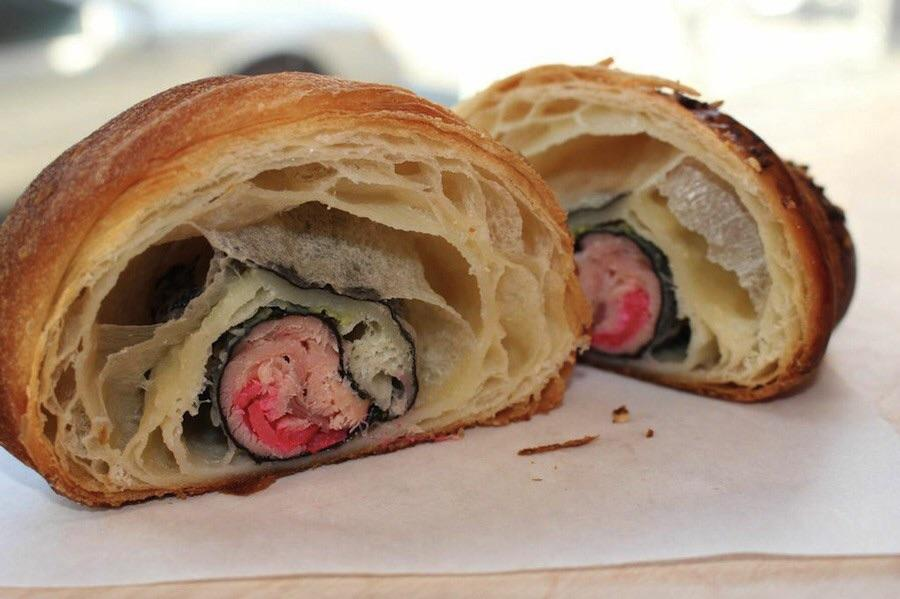
\includegraphics[scale=0.2]{img/croissant_sushi.png}
\end{figure}

\end{frame}




\end{document}